\documentclass[manuscript,screen,review,nonacm]{acmart}

\newcommand{\StudentName}{Your Name}
\newcommand{\StudentEmail}{your.email@university.edu}
\newcommand{\StudentUniversity}{Your University}
\newcommand{\StudentCity}{City}
\newcommand{\StudentState}{State}
\newcommand{\StudentCountry}{USA}
\newcommand{\CourseLine}{Course number and title, Fall 2026}

\usepackage{listings}
\usepackage{array}
\newcolumntype{L}[1]{>{\raggedright\arraybackslash}p{#1}}

\newcommand{\Shots}{8192}
\newcommand{\Seed}{2026}
\newcommand{\VerPython}{3.14.4}
\newcommand{\VerCirq}{1.7.0}
\newcommand{\VerQiskit}{2.5.2}
\newcommand{\VerAer}{0.17.2}
\newcommand{\VerNumpy}{2.5.3}
\newcommand{\VerScipy}{1.18.1}
\newcommand{\TbShots}{5000}
\newcommand{\TbExpectedX}{\ensuremath{0.1441}}
\newcommand{\TbPrintedX}{\ensuremath{0.2128}}
\newcommand{\TbAsPrintedX}{\ensuremath{0.2025}}
\newcommand{\TbFixedX}{\ensuremath{0.1441}}
\newcommand{\TbExpectedY}{\ensuremath{0.4132}}
\newcommand{\TbPrintedY}{\ensuremath{0.3746}}
\newcommand{\TbAsPrintedY}{\ensuremath{0.3876}}
\newcommand{\TbFixedY}{\ensuremath{0.4132}}
\newcommand{\TbExpectedZ}{\ensuremath{-0.8992}}
\newcommand{\TbPrintedZ}{\ensuremath{-0.8580}}
\newcommand{\TbAsPrintedZ}{\ensuremath{-0.8642}}
\newcommand{\TbFixedZ}{\ensuremath{-0.8992}}
\newcommand{\TbSigmaAsPrinted}{0.5}
\newcommand{\TbSigmaExpected}{3.4}
\newcommand{\TbClockAsPrintedLow}{0.89}
\newcommand{\TbClockAsPrintedHigh}{11.55}
\newcommand{\TbClockFixedLow}{1.00}
\newcommand{\TbClockFixedHigh}{13.00}
\newcommand{\TbSuccessAsPrinted}{0.259}
\newcommand{\TbAcceptedX}{1278}
\newcommand{\TbAcceptedY}{1292}
\newcommand{\TbAcceptedZ}{1296}
\newcommand{\TbReplayRuns}{100}
\newcommand{\TbReplaySigmaExpected}{27}
\newcommand{\TbReplaySigmaAsPrinted}{0.7}
\newcommand{\TbReplayX}{\ensuremath{0.203}}
\newcommand{\TbReplayY}{\ensuremath{0.388}}
\newcommand{\TbReplayZ}{\ensuremath{-0.865}}
\newcommand{\EOneNClock}{2}
\newcommand{\EOneLevels}{4}
\newcommand{\EOneQubits}{4}
\newcommand{\EOneT}{1.5708}
\newcommand{\EOneResolution}{1.000}
\newcommand{\EOneSuccessIdeal}{0.625}
\newcommand{\EOneSuccessExact}{0.625}
\newcommand{\EOneFidelity}{1.0000}
\newcommand{\EOneInfidelity}{\ensuremath{1.0\times 10^{-16}}}
\newcommand{\EOneRelErrExact}{0.0}
\newcommand{\EOneCx}{20}
\newcommand{\EOneDepth}{37}
\newcommand{\EOneAcceptedCirq}{5089}
\newcommand{\EOneSuccessCirq}{0.621}
\newcommand{\EOneAcceptedQiskit}{5159}
\newcommand{\EOneSuccessQiskit}{0.630}
\newcommand{\EOneEigLow}{1.000}
\newcommand{\EOneEigHigh}{2.000}
\newcommand{\EOneClockLow}{1.00}
\newcommand{\EOneClockHigh}{2.00}
\newcommand{\EOneErrorBar}{0.0078}
\newcommand{\ETwoNClock}{6}
\newcommand{\ETwoLevels}{64}
\newcommand{\ETwoQubits}{8}
\newcommand{\ETwoT}{1.5463}
\newcommand{\ETwoResolution}{0.063}
\newcommand{\ETwoSuccessIdeal}{0.464}
\newcommand{\ETwoSuccessExact}{0.454}
\newcommand{\ETwoFidelity}{0.9998}
\newcommand{\ETwoInfidelity}{\ensuremath{1.9\times 10^{-4}}}
\newcommand{\ETwoRelErrExact}{1.1}
\newcommand{\ETwoCx}{166}
\newcommand{\ETwoDepth}{243}
\newcommand{\ETwoAcceptedCirq}{3663}
\newcommand{\ETwoSuccessCirq}{0.447}
\newcommand{\ETwoAcceptedQiskit}{3739}
\newcommand{\ETwoSuccessQiskit}{0.456}
\newcommand{\ETwoEigLow}{1.382}
\newcommand{\ETwoEigHigh}{3.618}
\newcommand{\ETwoClockLow}{21.77}
\newcommand{\ETwoClockHigh}{56.98}
\newcommand{\ETwoErrorBar}{0.0276}
\newcommand{\EThreeNClock}{6}
\newcommand{\EThreeLevels}{64}
\newcommand{\EThreeQubits}{9}
\newcommand{\EThreeT}{1.2370}
\newcommand{\EThreeResolution}{0.079}
\newcommand{\EThreeSuccessIdeal}{0.500}
\newcommand{\EThreeSuccessExact}{0.495}
\newcommand{\EThreeFidelity}{0.9997}
\newcommand{\EThreeInfidelity}{\ensuremath{3.1\times 10^{-4}}}
\newcommand{\EThreeRelErrExact}{0.5}
\newcommand{\EThreeCx}{238}
\newcommand{\EThreeDepth}{370}
\newcommand{\EThreeAcceptedCirq}{4020}
\newcommand{\EThreeSuccessCirq}{0.491}
\newcommand{\EThreeAcceptedQiskit}{4078}
\newcommand{\EThreeSuccessQiskit}{0.498}
\newcommand{\EThreeEigLow}{1.382}
\newcommand{\EThreeEigHigh}{4.618}
\newcommand{\EThreeClockLow}{17.41}
\newcommand{\EThreeClockHigh}{58.19}
\newcommand{\EThreeErrorBar}{0.0110}
\newcommand{\EFourNClock}{6}
\newcommand{\EFourLevels}{64}
\newcommand{\EFourQubits}{9}
\newcommand{\EFourT}{1.2370}
\newcommand{\EFourResolution}{0.079}
\newcommand{\EFourSuccessIdeal}{0.168}
\newcommand{\EFourSuccessExact}{0.168}
\newcommand{\EFourFidelity}{0.9972}
\newcommand{\EFourInfidelity}{\ensuremath{2.8\times 10^{-3}}}
\newcommand{\EFourRelErrExact}{0.7}
\newcommand{\EFourCx}{262}
\newcommand{\EFourDepth}{418}
\newcommand{\EFourAcceptedCirq}{1401}
\newcommand{\EFourSuccessCirq}{0.171}
\newcommand{\EFourAcceptedQiskit}{1359}
\newcommand{\EFourSuccessQiskit}{0.166}
\newcommand{\EFourEigLow}{1.586}
\newcommand{\EFourEigHigh}{4.414}
\newcommand{\EFourClockLow}{19.98}
\newcommand{\EFourClockHigh}{55.62}
\newcommand{\EFourErrorBar}{0.0055}
\newcommand{\WorstSampledError}{3.3}
\newcommand{\WorstSigma}{2.6}
\newcommand{\NumSampledComponents}{22}
\newcommand{\FrameworkDifference}{\ensuremath{1.2\times 10^{-14}}}
\newcommand{\ETwoErrorFactor}{0.61}
\newcommand{\ETwoCxGrowth}{1.63}
\newcommand{\ETwoRelErrFour}{2.12}
\newcommand{\ETwoCxFour}{68}
\newcommand{\ETwoRelErrEight}{0.09}
\newcommand{\ETwoCxEight}{424}
\newcommand{\ETwoRelErrNine}{0.12}
\newcommand{\ETwoCxNine}{716}
\newcommand{\EThreeErrorFactor}{0.46}
\newcommand{\EThreeCxGrowth}{1.51}
\newcommand{\EThreeRelErrFour}{2.70}
\newcommand{\EThreeCxFour}{116}
\newcommand{\EThreeRelErrEight}{0.23}
\newcommand{\EThreeCxEight}{520}
\newcommand{\EThreeRelErrNine}{0.05}
\newcommand{\EThreeCxNine}{824}
\newcommand{\EFourErrorFactor}{0.52}
\newcommand{\EFourCxGrowth}{1.49}
\newcommand{\EFourRelErrFour}{1.93}
\newcommand{\EFourCxFour}{132}
\newcommand{\EFourRelErrEight}{0.10}
\newcommand{\EFourCxEight}{552}
\newcommand{\EFourRelErrNine}{0.12}
\newcommand{\EFourCxNine}{860}
\newcommand{\SweepMaxClock}{9}
\newcommand{\EOneCirqCountZeroZero}{0}
\newcommand{\EOneCirqCountZeroOne}{3103}
\newcommand{\EOneCirqCountOneZero}{4047}
\newcommand{\EOneCirqCountOneOne}{1042}
\newcommand{\EOneQiskitCountZeroZero}{0}
\newcommand{\EOneQiskitCountZeroOne}{3033}
\newcommand{\EOneQiskitCountOneZero}{4126}
\newcommand{\EOneQiskitCountOneOne}{1033}
\newcommand{\EOneCirqXOne}{0.994}
\newcommand{\EOneCirqXTwo}{0.504}
\newcommand{\ETwoAngle}{1.8546}
\newcommand{\ETwoPeakClock}{22}
\newcommand{\ETwoPeakProbability}{0.72}
\newcommand{\NumTests}{60}


\newcommand{\ket}[1]{\lvert #1\rangle}
\newcommand{\bra}[1]{\langle #1\rvert}
\newcommand{\norm}[1]{\lVert #1\rVert}
\newcommand{\code}[1]{\texttt{#1}}

\lstset{
  language=Python,
  basicstyle=\ttfamily\scriptsize,
  keywordstyle=\bfseries,
  commentstyle=\color{black!70},
  stringstyle=\color{black!80},
  showstringspaces=false,
  columns=fullflexible,
  keepspaces=true,
  breaklines=true,
  frame=lines,
  framesep=4pt,
  aboveskip=8pt,
  belowskip=4pt,
}

\begin{document}

\title[HHL in Cirq and Qiskit]{Solving Small Linear Systems with the HHL Algorithm:
  A Hands-On Tutorial in Cirq and Qiskit}
\subtitle{\CourseLine}

\author{\StudentName}
\email{\StudentEmail}
\affiliation{%
  \institution{\StudentUniversity}
  \city{\StudentCity}
  \state{\StudentState}
  \country{\StudentCountry}
}

\begin{abstract}
  The Harrow--Hassidim--Lloyd (HHL) algorithm prepares a quantum state whose
  amplitudes are proportional to the solution of a linear system $Ax=b$. This
  paper is a hands-on tutorial that builds the algorithm twice, in Cirq and in
  Qiskit, and runs it on four small systems taken from the statics of
  spring-coupled blocks: a diagonal $2\times 2$ system, a coupled $2\times 2$
  system whose eigenvalues are never used, a $4\times 4$ system, and a
  $3\times 3$ system padded to $4\times 4$. The Cirq version starts from a
  textbook listing that no longer runs on current Cirq; we document the
  repairs and show that one of them, an evolution time that is never handed to
  the solver, explains a mismatch in the textbook's printed output. The two
  free parameters of the algorithm are set from Gershgorin bounds instead of
  eigenvalues. On a noiseless simulator the two implementations agree to
  machine precision, and with six clock qubits and \Shots{} shots the sampled
  solutions lie within \WorstSampledError\,\% of the classical ones in
  Euclidean norm. Each additional clock qubit roughly halves the algorithmic
  error and multiplies the number of CNOT gates by 1.5 to 1.6. Throughout, we
  spell out how $A$ and $b$ enter the circuit and how measurement counts are
  turned back into numbers.
\end{abstract}

\begin{CCSXML}
<ccs2012>
 <concept>
  <concept_id>10003752.10003753.10003758</concept_id>
  <concept_desc>Theory of computation~Quantum computation theory</concept_desc>
  <concept_significance>500</concept_significance>
 </concept>
 <concept>
  <concept_id>10010520.10010521.10010542.10010550</concept_id>
  <concept_desc>Computer systems organization~Quantum computing</concept_desc>
  <concept_significance>500</concept_significance>
 </concept>
 <concept>
  <concept_id>10002950.10003705.10003707</concept_id>
  <concept_desc>Mathematics of computing~Solvers</concept_desc>
  <concept_significance>300</concept_significance>
 </concept>
</ccs2012>
\end{CCSXML}

\ccsdesc[500]{Theory of computation~Quantum computation theory}
\ccsdesc[500]{Computer systems organization~Quantum computing}
\ccsdesc[300]{Mathematics of computing~Solvers}

\keywords{quantum linear systems, HHL algorithm, quantum phase estimation,
  amplitude encoding, Cirq, Qiskit}

\maketitle

\section{Introduction}
\label{sec:intro}

Solving a system of linear equations $Ax=b$ is the workhorse of scientific
computing: finite-element models, circuit simulators and least-squares fits
all reduce to it. Classical solvers need time that grows at least linearly
with the number of unknowns $N$. In 2009 Harrow, Hassidim and Lloyd (HHL)
showed that, under certain conditions, a quantum computer can do the job in
time polynomial in $\log N$ and in the condition number $\kappa$ of $A$,
which is an exponential improvement in $N$ over the best classical
algorithms~\cite{harrow2009}.

The conditions matter~\cite{aaronson2015}. The vector $b$ has to be loaded
into a quantum state efficiently, the operator $e^{iAt}$ has to be
implemented efficiently, $\kappa$ must not be large, and the answer comes out
as a quantum state $\ket{x}$ instead of a list of numbers: each run of the
circuit yields a single sample, and learning all $N$ entries of $x$ takes
many runs. HHL is therefore best seen as a subroutine that hands $\ket{x}$ to
further quantum processing, and as the standard example of how phase
estimation can be turned into matrix arithmetic~\cite{dervovic2018}.

This paper is a tutorial. Reading about HHL is easier than implementing it.
The algorithm chains together state preparation, Hamiltonian evolution, phase
estimation, a controlled rotation, uncomputation and post-selection, and every
link has a bit order, a sign or a scaling constant that has to match its
neighbours. Our goal is to make each of these choices explicit, on systems
small enough to check by hand, and in two frameworks so that one
implementation can be tested against the other. The paper contributes the
following.
\begin{itemize}
\item A working Cirq implementation, obtained by repairing and extending the
  HHL listing of Pattanayak's textbook~\cite{pattanayak2021}. Every change is
  documented (Section~\ref{sec:cirq}), including the diagnosis of a mismatch
  between the numbers the listing expects and the numbers the book prints
  (Section~\ref{sec:textbook}).
\item An independent Qiskit implementation written from scratch
  (Section~\ref{sec:qiskit}). The two programs agree to within
  \FrameworkDifference{} on every exact output probability.
\item A recipe for choosing the two free parameters of HHL, the evolution
  time $t$ and the rotation constant $C$, from cheap eigenvalue bounds instead
  of the eigenvalues themselves (Section~\ref{sec:parameters}).
\item An explicit decoding rule that turns measurement counts into the
  entries of $x$ with error bars, including the norm $\norm{x}$ that the
  normalised quantum state seems to have lost (Section~\ref{sec:readout}).
\item Experiments on four linear systems up to $4\times 4$, and a study of
  how accuracy and gate count change with the size of the clock register
  (Section~\ref{sec:experiments}).
\end{itemize}
Section~\ref{sec:background} reviews the algorithm, Section~\ref{sec:encoding}
explains how a concrete linear system is encoded, Section~\ref{sec:implementation}
describes the two programs, and Section~\ref{sec:discussion} collects the
lessons we would pass on to the next student.

\section{Background}
\label{sec:background}

\subsection{Qubits, amplitudes and measurement}

A register of $q$ qubits is described by $2^q$ complex numbers, the
\emph{amplitudes}, one for each bit string of length $q$. We write the state
as $\sum_i a_i\ket{i}$ with $\sum_i |a_i|^2=1$, where $\ket{i}$ stands for the
$i$-th bit string in counting order ($0\dots00$, $0\dots01$, and so on). Gates
are unitary matrices acting on the vector of amplitudes. A measurement returns
bit string $i$ with probability $|a_i|^2$ and nothing else; in particular it
never shows an amplitude directly. Two consequences shape everything below:
a vector of $N$ numbers fits into only $\log_2 N$ qubits, and the only way to
learn about those numbers is to repeat the experiment and count
outcomes~\cite{nielsen2010}.

\subsection{What ``solving'' means on a quantum computer}

Let $A$ be an $N\times N$ Hermitian matrix with $N=2^m$. It has real
eigenvalues $\lambda_j$ and orthonormal eigenvectors $\ket{u_j}$, so
$A=\sum_j \lambda_j \ket{u_j}\bra{u_j}$. Expanding the normalised right-hand
side in the same basis, $\ket{b}=\sum_j\beta_j\ket{u_j}$, gives
\begin{equation}
  A^{-1}\ket{b} \;=\; \sum_j \frac{\beta_j}{\lambda_j}\,\ket{u_j}.
  \label{eq:inverse}
\end{equation}
Solving the system is nothing more than dividing every eigen-component of $b$
by its eigenvalue. HHL performs this division without being told the
eigenvalues or eigenvectors, and outputs the normalised state
$\ket{x}=A^{-1}\ket{b}/\norm{A^{-1}\ket{b}}$. If $A$ is not Hermitian one
solves the enlarged Hermitian system with matrix
$\bigl(\begin{smallmatrix}0&A\\A^\dagger&0\end{smallmatrix}\bigr)$
instead~\cite{harrow2009}; if $N$ is not a power of two the system is padded
(Section~\ref{sec:encodingA}).

\subsection{Quantum phase estimation}
\label{sec:qpe}

Phase estimation (QPE) is the tool that reads eigenvalues. Given a unitary
$U$ and one of its eigenvectors, $U\ket{u}=e^{2\pi i\varphi}\ket{u}$, QPE
writes an $n$-bit approximation of $\varphi$ into an $n$-qubit \emph{clock}
register: Hadamard gates put the clock into a uniform superposition, clock
qubit $j$ then controls $U^{2^j}$, and an inverse quantum Fourier transform
(QFT) converts the accumulated phases into a binary
number~\cite{cleve1998,nielsen2010}. For HHL we take $U=e^{iAt}$, whose
eigenvectors are those of $A$ and whose phases are
$\varphi_j=\lambda_j t/2\pi$. The clock then holds the integer
\begin{equation}
  k_j \;=\; 2^n\varphi_j \;=\; \frac{\lambda_j\,t\,2^n}{2\pi}.
  \label{eq:clock}
\end{equation}
If $k_j$ is an integer the clock ends exactly in $\ket{k_j}$. If not, the
outcome is spread over the integers around $k_j$; the nearest one still has
probability at least $4/\pi^2\approx 0.41$~\cite{cleve1998}. This spreading is
the only approximation in the circuits of this paper, and
Section~\ref{sec:sweep} measures its effect. Because QPE is linear, running it
on $\ket{b}$ treats all eigen-components at once and produces
$\sum_j\beta_j\ket{k_j}\ket{u_j}$.

\subsection{The five stages of HHL}
\label{sec:stages}

\begin{figure}[t]
  \centering
  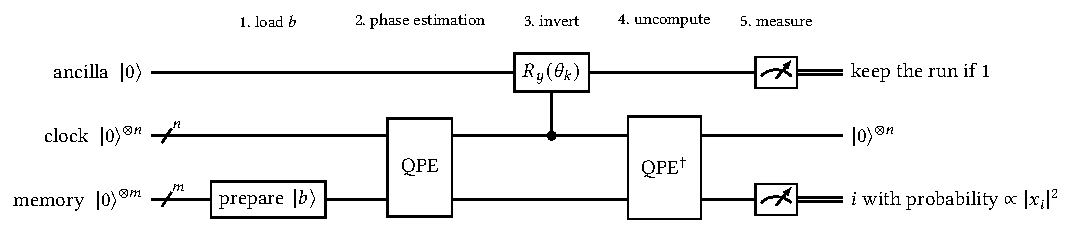
\includegraphics[width=\linewidth]{figures/fig_hhl_schematic}
  \caption{The HHL circuit. The memory register holds $\ket{b}$ at the start
    and $\ket{x}$ at the end, the clock register temporarily stores the
    eigenvalues, and one ancilla qubit carries the factor $1/\lambda$.}
  \Description{Circuit diagram with three horizontal wires labelled ancilla,
    clock and memory. From left to right: a state preparation box on the
    memory, a phase estimation box spanning clock and memory, a rotation on
    the ancilla controlled by the clock, an inverse phase estimation box, and
    measurements of the ancilla and the memory.}
  \label{fig:schematic}
\end{figure}

Figure~\ref{fig:schematic} shows the circuit. It uses three registers: an
ancilla qubit, the $n$-qubit clock and the $m$-qubit memory. Writing the
registers in that order, the state evolves as follows.
\begin{enumerate}
\item \emph{Load $b$.} The memory is prepared in $\ket{b}$:
  $\;\ket{0}\ket{0}\ket{b}$.
\item \emph{Phase estimation.} The eigenvalues are written into the clock:
  $\;\ket{0}\sum_j\beta_j\ket{k_j}\ket{u_j}$.
\item \emph{Eigenvalue inversion.} The ancilla is rotated about the $y$ axis
  by an angle that depends on the clock value, $\theta_k=2\arcsin(C/\lambda_k)$,
  where $\lambda_k$ is the eigenvalue that clock value $k$ stands for. Since
  $R_y(\theta)\ket{0}=\cos\tfrac{\theta}{2}\ket{0}+\sin\tfrac{\theta}{2}\ket{1}$,
  this gives
  \begin{equation}
    \sum_j\beta_j\Bigl(\sqrt{1-C^2/\lambda_j^2}\,\ket{0}
      +\frac{C}{\lambda_j}\ket{1}\Bigr)\ket{k_j}\ket{u_j}.
    \label{eq:rotation}
  \end{equation}
\item \emph{Uncompute.} Phase estimation is run backwards, which returns the
  clock to $\ket{0}$ and removes the labels $\ket{k_j}$.
\item \emph{Measure.} The ancilla is measured. With probability
  \begin{equation}
    p_1 \;=\; C^2\sum_j\frac{|\beta_j|^2}{\lambda_j^2}
        \;=\; C^2\,\norm{A^{-1}\ket{b}}^2
    \label{eq:psuccess}
  \end{equation}
  the outcome is 1, and the memory is then left in
  $\sum_j(\beta_j/\lambda_j)\ket{u_j}$ up to normalisation, which is
  $\ket{x}$ by Eq.~\eqref{eq:inverse}. Runs with outcome 0 are discarded.
\end{enumerate}
Stage~4 is easy to overlook and essential. Without it every term in the
memory would still be tagged by its own clock state $\ket{k_j}$, the terms
could not interfere, and measuring the memory would give the probabilities of
a mixture of eigenvectors instead of those of the single vector
$\sum_j(\beta_j/\lambda_j)\ket{u_j}$.

\subsection{Cost and fine print}

For an $s$-sparse matrix, HHL prepares $\ket{x}$ to precision $\epsilon$ in
time $\tilde{O}(\log(N)\,s^2\kappa^2/\epsilon)$~\cite{harrow2009}; later
algorithms improve the dependence on $\epsilon$ to
polylogarithmic~\cite{childs2017}. Even for the largest allowed $C$ the success
probability $p_1$ can be as small as $1/\kappa^2$; amplitude amplification
reduces the number of repetitions this costs from about $\kappa^2$ to about
$\kappa$~\cite{brassard2002,harrow2009}. None of this helps if loading
$b$ or reading out $x$ costs time proportional to $N$~\cite{aaronson2015}.
In a simulation of a $4\times 4$ system none of these costs bite, but each of
them leaves a visible trace in our code, and we point them out as they appear.

\section{Encoding a linear system into a circuit}
\label{sec:encoding}

\subsection{The test problems}

\begin{figure}[t]
  \centering
  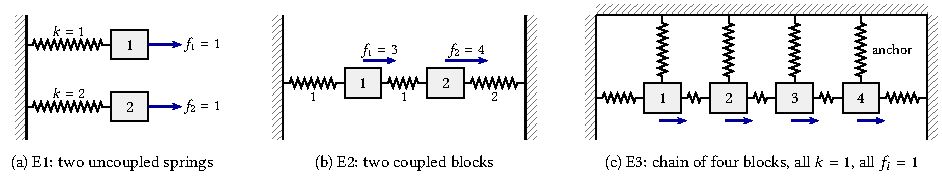
\includegraphics[width=\linewidth]{figures/fig_springs}
  \caption{The mechanical systems behind the experiments. Blocks slide
    horizontally; $k$ is a spring stiffness and $f_i$ the force applied to
    block $i$. In (c) every block is also tied to a fixed frame by an anchor
    spring, drawn vertically to keep the picture readable; it pulls block $i$
    back with force $x_i$. Experiment E4 uses the same chain with three
    blocks and a force on the first block only.}
  \Description{Three drawings of blocks connected by springs. Panel a: two
    separate blocks, each attached to a wall by its own spring with stiffness
    1 and 2, each pulled by a unit force. Panel b: two blocks between two
    walls joined by three springs of stiffness 1, 1 and 2, with forces 3 and
    4. Panel c: four blocks in a row between two walls, joined by unit
    springs, each also attached to a rail above by an anchor spring, each
    pushed by a unit force.}
  \label{fig:springs}
\end{figure}

We wanted examples whose answers can be checked by intuition as well as by
NumPy, so all four systems describe blocks connected by springs
(Figure~\ref{fig:springs}). If block $i$ is displaced by $x_i$ and pushed by a
force $f_i$, balance of forces gives the linear system $Kx=f$. The
\emph{stiffness matrix} $K$ carries on its diagonal the total stiffness of all
springs attached to a block and off the diagonal minus the stiffness of the
spring joining two blocks:
\begin{equation}
  K_{\mathrm{E1}}=\begin{pmatrix}1&0\\0&2\end{pmatrix},\qquad
  K_{\mathrm{E2}}=\begin{pmatrix}2&-1\\-1&3\end{pmatrix},\qquad
  K_{\mathrm{E3}}=\begin{pmatrix}3&-1&0&0\\-1&3&-1&0\\0&-1&3&-1\\0&0&-1&3\end{pmatrix}.
  \label{eq:matrices}
\end{equation}
In HHL's notation $A=K$ and $b=f$.
\begin{description}
\item[E1, two uncoupled springs.] $f=(1,1)$, so $x=(1,\tfrac12)$: the stiffer
  spring stretches half as far. The matrix is diagonal, its eigenvectors are
  the basis states $\ket{0}$ and $\ket{1}$ and its eigenvalues can be read
  off, so every step of the algorithm can be checked by hand.
\item[E2, two coupled blocks.] $f=(3,4)$ and $x=(2.6,\,2.2)$. The off-diagonal
  entry couples the blocks, the eigenvalues $(5\mp\sqrt5)/2$ are irrational,
  and our code never uses them.
\item[E3, chain of four blocks.] $f=(1,1,1,1)$ and $x=(0.6,\,0.8,\,0.8,\,0.6)$:
  the blocks next to the walls move less than the two in the middle.
\item[E4, chain of three blocks.] The $3\times 3$ version of $K_{\mathrm{E3}}$
  with $f=(1,0,0)$ and $x=(8,3,1)/21\approx(0.381,\,0.143,\,0.048)$: a push on
  the first block dies out along the chain. Three is not a power of two, so
  this system is padded to $4\times 4$.
\end{description}
Stiffness matrices of this kind have two convenient properties. They are
symmetric and positive definite, so they are Hermitian with positive
eigenvalues. And because their off-diagonal entries are never positive, their
inverses have no negative entries~\cite{berman1994}: pushing blocks to the
right never moves a block to the left. We will use the second fact when
reading out the solution, because a measurement only reveals $|x_i|$.

\subsection{Encoding \texorpdfstring{$b$}{b}: amplitude encoding}
\label{sec:encodingb}

The right-hand side becomes the amplitudes of the memory register,
\begin{equation}
  \ket{b}=\frac{1}{\norm{b}}\sum_{i=1}^{N} b_i\ket{i},
\end{equation}
so the first entry sits on the bit string of all zeros, the second on
$0\dots01$, and so on. A quantum state has unit length, so the length
$\norm{b}$ is not stored in the circuit; we keep it on paper and multiply it
back in at the end (Section~\ref{sec:readout}). For one qubit a single rotation
does the job, since
$R_y(\theta)\ket{0}=\cos\tfrac{\theta}{2}\ket{0}+\sin\tfrac{\theta}{2}\ket{1}$:
\begin{equation}
  \theta=2\,\mathrm{atan2}(b_2,b_1).
\end{equation}
For E1 this is $\theta=\pi/2$, the same state a Hadamard gate would give. For
E2 the forces $(3,4)$ have length 5, the amplitudes are $(0.6,\,0.8)$ and
$\theta=2\arctan(4/3)=\ETwoAngle$~rad.

For more qubits the same idea is applied recursively~\cite{mottonen2005,shende2006}.
The first qubit is rotated so that the probability of finding it in 0 or 1
equals the weight of the upper and the lower half of $b$. The second qubit
then splits each half again, with one rotation angle for each value of the
first qubit, and so on down a binary tree. Signs are taken care of in the last
level by using the signed entries in the $\mathrm{atan2}$. Our Cirq code
builds this tree by hand (\code{amplitude\_encoding}); in Qiskit the library
gate \code{StatePreparation} does the same. For E3 the tree reduces to
$R_y(\pi/2)$ on both qubits, and for E4 to no gate at all, because
$(1,0,0,0)$ is the state $\ket{00}$ the register starts in. A general vector
needs on the order of $N$ rotations, which is the first piece of fine print:
HHL only pays off if $b$ has enough structure to be loaded faster.

\subsection{Encoding \texorpdfstring{$A$}{A}: a time evolution}
\label{sec:encodingA}

The matrix does not appear in the circuit as a table of numbers. It enters
through the unitary $U=e^{iAt}$, and only in the controlled powers
$U^{2^j}$ that phase estimation needs. On a quantum computer these would be
produced by a Hamiltonian-simulation routine that exploits the sparsity of
$A$~\cite{lloyd1996,berry2007}. On a simulator we take a shortcut: the
$2^m\times 2^m$ matrix $U$ is computed classically (the textbook listing
diagonalises $A$, our Qiskit code calls a matrix exponential) and inserted as
a single gate. This shortcut costs as much as solving the system classically,
so it says nothing about speed. What it preserves is the logic of the
algorithm, provided that the eigenvalues are not used anywhere else, and the
next subsection makes sure of that.

When $N$ is not a power of two, $A$ is embedded in the next larger matrix
with a constant $\lambda_{\mathrm{pad}}$ on the new diagonal entries and zeros
elsewhere, and $b$ is extended by zeros. The solution of the padded system is
$(x,0,\dots,0)$. For E4 we use $\lambda_{\mathrm{pad}}=3$, the value of the
other diagonal entries; any value inside the eigenvalue bounds of the next
subsection works.

\subsection{Choosing \texorpdfstring{$t$ and $C$}{t and C} without knowing the eigenvalues}
\label{sec:parameters}

HHL has two free parameters. The evolution time $t$ sets the scale of the
clock: by Eq.~\eqref{eq:clock}, clock value $k$ stands for the eigenvalue
\begin{equation}
  \lambda_k=\frac{2\pi k}{2^n t},\qquad k=1,\dots,2^n-1.
  \label{eq:lambdak}
\end{equation}
Phases are periodic, so an eigenvalue above $2\pi/t$ would wrap around and be
mistaken for a small one. The constant $C$ scales the rotation of
Eq.~\eqref{eq:rotation}; the amplitude $C/\lambda$ cannot exceed 1, so $C$
must not be larger than the smallest eigenvalue. Both requirements ask for
bounds on the spectrum, not for the spectrum itself:
\begin{equation}
  C\le\lambda_{\min},\qquad \lambda_{\max}\le\Lambda,\qquad
  t=\frac{2\pi}{\Lambda}\,\frac{2^n-1}{2^n}.
  \label{eq:tchoice}
\end{equation}
With this $t$ the upper bound $\Lambda$ sits on the last clock value
$2^n-1$, and neighbouring clock values are $\Lambda/(2^n-1)$ apart.

Bounds of this kind are cheap. By the Gershgorin circle theorem every
eigenvalue of $A$ lies in at least one of the intervals
$[a_{ii}-R_i,\;a_{ii}+R_i]$ with $R_i=\sum_{j\ne i}|a_{ij}|$~\cite{horn2012},
which takes one pass over the entries of the matrix. For $K_{\mathrm{E2}}$
the two rows give $[1,3]$ and $[2,4]$, hence $C=1$ and $\Lambda=4$; the true
eigenvalues, $1.38$ and $3.62$, lie inside as they must. For the two chains the
rows give $[2,4]$ and $[1,5]$, hence $C=1$ and $\Lambda=5$.
Listing~\ref{lst:parameters} shows the corresponding code.

\lstinputlisting[float=t,caption={Choosing the parameters and the rotation
  angles from eigenvalue bounds (\code{hhl\_common.py}). Both implementations
  read their angles from this one table.},label={lst:parameters}]{code/excerpt_parameters.py}

Three details of Listing~\ref{lst:parameters} deserve a comment.

\emph{Clock value zero.} Following the textbook listing, $k=0$ is read as
$k=2^n$, that is, as the eigenvalue $2\pi/t$ just above $\Lambda$. Since
phases are periodic, an eigenvalue close to $\Lambda$ leaks to $k=0$ as easily
as to $k=2^n-2$, and this convention gives the leaked amplitude a sensible
weight.

\emph{The textbook's default for $C$.} The listing sets $C$ to the smallest
eigenvalue the clock can represent, $C=\lambda_1=2\pi/(2^n t)$. This is always
allowed, but it ties $C$ to the resolution of the clock: each extra clock qubit
halves $C$ and, by Eq.~\eqref{eq:psuccess}, divides the success probability by
four. Taking $C$ from a lower bound on the eigenvalues keeps the success
probability independent of $n$.

\emph{Clock values below $C$.} Once $C$ is larger than $\lambda_1$, some clock
values stand for eigenvalues smaller than $C$, for which $\arcsin(C/\lambda_k)$
does not exist. If $C$ really is a lower bound, no eigenvalue of $A$ lives
there, and any amplitude found on those clock values has leaked in from phase
estimation. We leave the ancilla untouched in that case (angle 0), in the
spirit of the filter functions of the original paper~\cite{harrow2009}.

The Gershgorin lower bound is positive only if every diagonal entry exceeds
the sum of the absolute values of the other entries in its row. This holds for
our spring systems because every block is tied to something fixed. For other
matrices one has to bound $\lambda_{\min}$ by other means (the original
algorithm assumes that $\kappa$ is known~\cite{harrow2009}) or fall back on the
textbook default. Table~\ref{tab:parameters} lists the parameters of the
four experiments. For E1, where the eigenvalues $1$ and $2$ are visible in the
matrix, we chose $\Lambda=3$ by hand so that with two clock qubits clock value
$k$ stands exactly for the eigenvalue $k$.

\begin{table}[t]
  \caption{The four experiments. $C$ and $\Lambda$ are the lower and upper
    eigenvalue bounds, $n$ the number of clock qubits and $t$ the evolution
    time of Eq.~\eqref{eq:tchoice}. The qubit count includes the ancilla.}
  \label{tab:parameters}
  \small
  \begin{tabular}{llccclccc}
\toprule
 & System & Size & $b$ & $[C,\Lambda]$ & Bounds from & $n$ & $t$ & Qubits \\
\midrule
E1 & Two uncoupled springs & $2\times2$ & $(1,1)$ & $[1,\,3]$ & by inspection & 2 & $1.5708$ & 4 \\
E2 & Two coupled blocks & $2\times2$ & $(3,4)$ & $[1,\,4]$ & Gershgorin & 6 & $1.5463$ & 8 \\
E3 & Chain of four blocks & $4\times4$ & $(1,1,1,1)$ & $[1,\,5]$ & Gershgorin & 6 & $1.2370$ & 9 \\
E4 & Chain of three blocks & $3\times3$ (padded) & $(1,0,0)$ & $[1,\,5]$ & Gershgorin & 6 & $1.2370$ & 9 \\
\bottomrule
\end{tabular}

\end{table}

\section{Implementation}
\label{sec:implementation}

\subsection{Cirq: from the textbook listing to a working program}
\label{sec:cirq}

\begin{sloppypar}
Listing~5.1 of Pattanayak's book~\cite{pattanayak2021} implements HHL for a
$2\times 2$ matrix in Cirq~\cite{cirq}. It is closely related to the HHL
example distributed with Cirq~\cite{cirqhhl}, with which it shares its test
matrix and its rotation code, and which in turn cites the survey of Abhijith
et~al.~\cite{abhijith2022}. The listing splits the program into classes that
mirror Figure~\ref{fig:schematic}. The class \code{HamiltonianSimulation}
provides $U=e^{-iAt}$ as a Cirq \code{EigenGate}. The classes
\code{ControlledUnitary} and \code{QuantumPhaseEstimation} build stage~2, and
\code{EigenValueInversion} is stage~3. The class \code{HHL} assembles the
circuit and measures the Pauli observables $\langle X\rangle$,
$\langle Y\rangle$ and $\langle Z\rangle$ of the memory qubit.
\end{sloppypar}

The listing was written for Cirq~0.8.2 and does not run on the current
release (\VerCirq). Table~\ref{tab:repairs} lists what we changed. The first
two rows are needed before the program starts at all. The third is the
interesting one: the script defines the evolution time
$t=0.358166\,\pi$, then creates the solver without it,
\begin{lstlisting}[frame=none,aboveskip=4pt,belowskip=4pt]
_hhl_ = HHL(hamiltonian=A, initial_state_transforms=initial_state_transforms,
            qpe_register_size=4)                  # as printed: t falls back to 1
_hhl_ = HHL(hamiltonian=A, initial_state_transforms=initial_state_transforms,
            qpe_register_size=4, t=t)             # corrected
\end{lstlisting}
so the constructor's default $t=1$ is used. Nothing crashes; the circuit is
simply built for the wrong time. Section~\ref{sec:textbook} shows that this
accounts for the numbers printed in the book.

\begin{table}[t]
  \caption{Changes made to the textbook listing. ``Listing'' refers to the
    files as printed, run with Cirq~\VerCirq.}
  \label{tab:repairs}
  \small
  \begin{tabular}{p{0.3cm}L{4.9cm}L{4.2cm}L{4.3cm}}
    \toprule
     & In the listing & Effect & Our change \\
    \midrule
    1 & \code{HamiltonianSimulation} inherits from \code{cirq.SingleQubitGate}
      & \code{AttributeError} on import; the class was removed from Cirq
      & define \code{\_num\_qubits\_}, which also lifts the restriction to one qubit \\
    2 & imports a \code{QFT} class from Chapter~4 of the book
      & needed to build phase estimation
      & rebuilt gate by gate from the circuit diagram in the book's output \\
    3 & \code{HHL(...)} is created without \code{t}
      & runs with $t=1$; eigenvalues fall between clock values and the result is biased
      & pass \code{t=t} \\
    4 & rotation angle computed as \code{asin(C*N*t/(2*pi*k))}
      & \code{ValueError} (math domain error) as soon as $C>\lambda_1$
      & shared angle table with the cut-off of Section~\ref{sec:parameters} \\
    5 & memory register is a single qubit
      & only $2\times 2$ systems
      & $m$ memory qubits, amplitude encoding, counts over all basis states \\
    6 & unused \code{main()} that calls undefined names; a method \code{circuit()}
        that overwrites itself; debugging prints
      & harmless but confusing
      & removed or simplified; readable labels in circuit diagrams \\
    \bottomrule
  \end{tabular}
\end{table}

Two conventions of the listing are worth knowing because they differ from
most textbooks. First, its clock register is big-endian: the first clock qubit
is the most significant bit and controls the highest power $U^{2^{n-1}}$.
Second, it evolves with $U=e^{-iAt}$ and compensates with a Fourier transform
of the opposite sign: what the book calls the QFT multiplies by
$e^{-2\pi i xy/2^n}$, and phase estimation applies its inverse. We confirmed
this by comparing the rebuilt circuit with the discrete Fourier transform
matrix. The combination stores the same integer $k_j$ as
Eq.~\eqref{eq:clock}.

\lstinputlisting[float=t,caption={Eigenvalue inversion in Cirq, adapted from
  the textbook listing (\code{hhl\_cirq.py}). The argument \code{qubits} holds
  the clock qubits followed by the ancilla.},label={lst:inversion}]{code/excerpt_cirq_inversion.py}

Listing~\ref{lst:inversion} shows how the listing implements stage~3. A
controlled gate acts when all its control qubits are 1. To make it act on
clock value $k$, the clock qubits that are 0 in the binary form of $k$ are
flipped with $X$ gates first. Going through $k=0,1,2,\dots$ in order, only the
bits in which $k$ and $k-1$ differ need to be flipped between two rotations,
and after the last value all flips have cancelled. The result is one
multi-controlled $R_y$ for every clock value that is allowed to rotate the
ancilla.

\subsection{Qiskit: written from scratch}
\label{sec:qiskit}

Qiskit~\cite{qiskit2024} used to include an \code{HHL} class, but it was
deprecated and removed together with the other linear solvers of
\code{qiskit.algorithms}~\cite{qiskitmigration}, so the circuit has to be
assembled by hand. Listing~\ref{lst:qiskit} is the core of our
implementation; it was written with the help of an AI assistant (see the
acknowledgments).

\lstinputlisting[float=t,caption={The HHL circuit in Qiskit
  (\code{hhl\_qiskit.py}).},label={lst:qiskit}]{code/excerpt_qiskit_circuit.py}

The code reads like Figure~\ref{fig:schematic}. Phase estimation is built as a
sub-circuit so that stage~4 is one call to \code{inverse()}. Stage~3 is a
single library gate: a \emph{uniformly controlled rotation} \code{UCRYGate}
takes a list of $2^n$ angles and applies the $k$-th one when its control
qubits hold the value $k$. It is a look-up table in gate form and compiles to
$2^n$ CNOT gates and $2^n$ single-qubit rotations~\cite{mottonen2005}, which
is cheaper than the $2^n$ multi-controlled rotations of
Listing~\ref{lst:inversion}.

Qiskit's conventions are the opposite of the listing's in almost every
respect (Table~\ref{tab:conventions}). Registers are little-endian, so
\code{clock[j]} controls $U^{2^j}$, and we use the textbook form of phase
estimation, $U=e^{+iAt}$ followed by the inverse QFT. The two programs
nevertheless prepare the same state. We did not take that on faith: for all
four experiments and for every clock size in Section~\ref{sec:sweep} the exact
output probabilities of the two programs differ by at most
\FrameworkDifference.

\begin{table}[t]
  \caption{Conventions of the two implementations.}
  \label{tab:conventions}
  \small
  \begin{tabular}{L{3.3cm}L{5.3cm}L{5.3cm}}
    \toprule
     & Cirq (from the listing) & Qiskit (ours) \\
    \midrule
    Bit order in a register & first qubit is the most significant bit
      & first qubit is the least significant bit \\
    Evolution operator & $U=e^{-iAt}$ & $U=e^{+iAt}$ \\
    Clock qubit $j$ controls & $U^{2^{\,n-1-j}}$ & $U^{2^{\,j}}$ \\
    Transform after the controlled powers & phases $e^{+2\pi i xy/2^n}$
      (the listing's ``inverse QFT'') & phases $e^{-2\pi i xy/2^n}$
      (inverse of \code{QFTGate}) \\
    Construction of $U$ & eigendecomposition inside a \code{cirq.EigenGate}
      & \code{scipy.linalg.expm}, wrapped in a \code{UnitaryGate} \\
    Loading $b$ & tree of controlled $R_y$ gates, written by hand
      & \code{StatePreparation} \\
    Eigenvalue inversion & multi-controlled $R_y$ per clock value, selected
      with $X$ gates & one \code{UCRYGate} (look-up table) \\
    Exact statistics & \code{cirq.Simulator().simulate}
      & \code{qiskit.quantum\_info.Statevector} \\
    Sampling & \code{cirq.Simulator().run} & \code{AerSimulator().run} \\
    Printed outcomes & one array per measurement key
      & bit string, last classical bit first \\
    \bottomrule
  \end{tabular}
\end{table}

\subsection{Reading out the solution}
\label{sec:readout}

At the end of the circuit we measure the ancilla and the memory and count how
often each combination occurs. Let $n(a,i)$ be the number of shots, out of $S$,
in which the ancilla showed $a$ and the memory showed its $i$-th basis state. Only
$a=1$ matters. Combining Eq.~\eqref{eq:psuccess} with the fact that
$A^{-1}\ket{b}=x/\norm{b}$, the probability of the pair $(1,i)$ is
\begin{equation}
  P(1,i)=\frac{C^2}{\norm{b}^2}\,x_i^2
  \qquad\Longrightarrow\qquad
  |x_i|\;\approx\;\frac{\norm{b}}{C}\sqrt{\frac{n(1,i)}{S}}.
  \label{eq:decode}
\end{equation}
This one formula is the whole interpretation step, and three remarks complete
it.

\emph{The norm is not lost.} A normalised state cannot hold $\norm{x}$, but the
success rate can: summing Eq.~\eqref{eq:decode} over $i$ gives
$\norm{x}\approx(\norm{b}/C)\sqrt{n_1/S}$, where $n_1$ is the number of
accepted shots. The discarded runs are not wasted; their fraction is a
measurement.

\emph{Error bars.} Each count is binomial, so the standard error of
$\hat p=n(1,i)/S$ is $\sqrt{\hat p(1-\hat p)/S}$, and propagating it through
the square root gives
\begin{equation}
  \delta|x_i|=\frac{\norm{b}}{C}\sqrt{\frac{1-\hat p}{4S}}
  \;\le\;\frac{\norm{b}}{2C\sqrt{S}}.
  \label{eq:errorbar}
\end{equation}
The absolute uncertainty is roughly the same for every entry, so small entries
are the hardest to measure in relative terms. All $\pm$ values in this paper
are one standard error computed in this way.

\emph{Signs.} Eq.~\eqref{eq:decode} only gives magnitudes. For our spring
systems this is enough, because all displacements are known to be non-negative
(Section~\ref{sec:encoding}). In general, relative signs and phases need
additional measurements in other bases. For a one-qubit memory the textbook
listing does this by measuring the three Pauli observables: if
$\ket{x}=\tilde x_1\ket{0}+\tilde x_2\ket{1}$, then
$\langle Z\rangle=|\tilde x_1|^2-|\tilde x_2|^2$ fixes the magnitudes and
$\langle X\rangle=2\,\mathrm{Re}(\tilde x_1^{*}\tilde x_2)$ and
$\langle Y\rangle=2\,\mathrm{Im}(\tilde x_1^{*}\tilde x_2)$ fix the relative
phase. We keep this read-out for the $2\times 2$ experiments. A positive
$\langle X\rangle$ together with $\langle Y\rangle=0$ means that the two
entries are real with the same sign.

On a simulator there is a second way to look at the result: the final state
vector gives the probabilities $P(1,i)$ exactly, without shot noise. We report
both, the ``exact circuit'' values to show what the algorithm itself gets
wrong, and sampled values to show what an experiment would see. From the state
vector we also compute the fidelity $F=\bra{x}\rho\ket{x}$ between the
classical solution and the state $\rho$ of the memory after a successful run.

\subsection{Testing}

Both programs come with \NumTests{} automated tests. They compare each
building block with plain NumPy (the evolution gate with a matrix
exponential, the Fourier transform with its matrix, the clock contents and
rotation angles with their formulas), each complete solver with
\code{numpy.linalg.solve}, and the two frameworks with each other. As a check
that does not depend on either framework, the five stages of
Section~\ref{sec:stages} are also written out as plain matrix algebra in about
twenty lines of NumPy; both circuits reproduce its output probabilities. All
figures, tables and numbers quoted in this paper are generated from one results
file by a script, so nothing was copied by hand.

\begin{figure}[t]
  \centering
  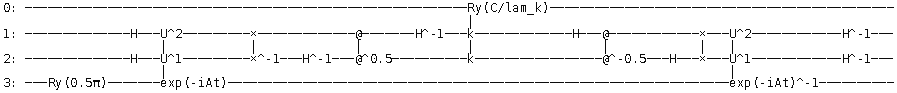
\includegraphics[width=\linewidth]{figures/fig_circuit_cirq}\\[8pt]
  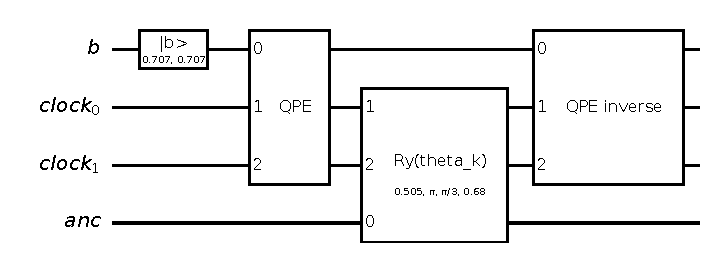
\includegraphics[height=3.4cm]{figures/fig_circuit_qiskit}\hfill
  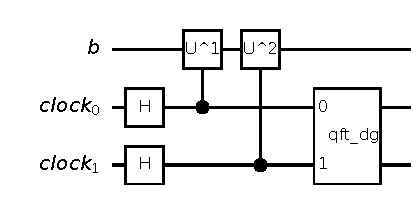
\includegraphics[height=2.65cm]{figures/fig_circuit_qiskit_qpe}
  \caption{The circuit of experiment E1 as drawn by each framework. Top: Cirq,
    with the ancilla on line 0, the clock on lines 1 and 2 and the memory on
    line 3; \code{H\^{}-1} and \code{x\^{}-1} are the inverses of the Hadamard
    and swap gates, which equal the gates themselves. Bottom left: Qiskit, with
    the memory on top and the angles $\theta_0,\dots,\theta_3$ of the look-up
    rotation printed in the box. Bottom right: the inside of the QPE block.}
  \Description{Three circuit diagrams. The Cirq text diagram shows an Ry gate
    on the memory, Hadamard gates and controlled powers of the evolution
    operator on the clock, a Fourier transform, a rotation on the ancilla
    controlled by the clock, and the mirror image of the first half. The
    Qiskit diagram shows four boxes: state preparation, QPE, a rotation with
    angles 0.505, pi, pi over 3 and 0.68, and the inverse QPE. The third
    diagram shows two Hadamard gates, two controlled unitaries and an inverse
    Fourier transform.}
  \label{fig:circuits}
\end{figure}

\section{Experiments}
\label{sec:experiments}

\subsection{Setup}

All runs are noiseless simulations with Python~\VerPython, Cirq~\VerCirq,
Qiskit~\VerQiskit{} and Qiskit Aer~\VerAer. Each circuit is sampled \Shots{}
times. The random seed is fixed (\Seed) and the Qiskit circuits are compiled
without optimisation; with these two settings and the library versions above,
repeated runs reproduce every number in this paper exactly
(Section~\ref{sec:discussion} explains why the second setting is needed). The complete set of experiments takes well under a
minute on two CPU cores.

\subsection{Validation on the textbook example}
\label{sec:textbook}

The listing comes with its own test case: a $2\times 2$ Hermitian matrix with
eigenvalues $0.349$ and $4.537$, a complex $\ket{b}$ prepared by two
rotations, four clock qubits, and the expected values
$\langle X\rangle=\TbExpectedX$, $\langle Y\rangle=\TbExpectedY$ and
$\langle Z\rangle=\TbExpectedZ$ of the solution qubit. The time
$t=0.358166\,\pi$ is chosen so that the two eigenvalues land exactly on the
clock values $\TbClockFixedLow$ and $\TbClockFixedHigh$. The output printed in
the book, however, is $(\TbPrintedX,\ \TbPrintedY,\ \TbPrintedZ)$.

\begin{table}[t]
  \caption{The textbook example: Pauli expectation values of the solution
    qubit. ``Exact'' rows are computed from the state vector; sampled rows
    show one standard error.}
  \label{tab:textbook}
  \small
  \begin{tabular}{lccc}
\toprule
Source & $\langle X\rangle$ & $\langle Y\rangle$ & $\langle Z\rangle$ \\
\midrule
Expected values quoted in the listing & $0.1441$ & $0.4132$ & $-0.8992$ \\
Classical solution (NumPy) & $0.1441$ & $0.4132$ & $-0.8992$ \\
\midrule
Output printed in the book (5000 repetitions) & $0.2128$ & $0.3746$ & $-0.8580$ \\
Original listing, unmodified (mean of 100 runs) & $0.2025 \pm 0.0030$ & $0.3880 \pm 0.0023$ & $-0.8651 \pm 0.0013$ \\
Our port with $t$ not passed ($t=1$), exact & $0.2025$ & $0.3876$ & $-0.8642$ \\
\midrule
Our port with $t$ passed, exact & $0.1441$ & $0.4132$ & $-0.8992$ \\
Cirq with $t$ passed, 5000 repetitions & $0.145 \pm 0.027$ & $0.411 \pm 0.026$ & $-0.894 \pm 0.012$ \\
Qiskit with $t$ passed, 5000 repetitions & $0.131 \pm 0.027$ & $0.414 \pm 0.025$ & $-0.904 \pm 0.012$ \\
\bottomrule
\end{tabular}

\end{table}

Table~\ref{tab:textbook} resolves the discrepancy. To rule out our own port as
the cause, we first ran the original files unmodified, supplying the two
missing pieces of Table~\ref{tab:repairs} (rows 1 and 2) from outside. Averaged
over \TbReplayRuns{} runs they print $(\TbReplayX,\ \TbReplayY,\ \TbReplayZ)$,
which is \TbReplaySigmaExpected{} standard errors away from the values the
listing expects and matches, within \TbReplaySigmaAsPrinted{} standard errors,
the exact result of our port when $t$ is left at its default of 1. In the Cirq
example the time is passed to the circuit; the argument was lost when the code
was reorganised into classes. With $t=1$ the eigenvalues correspond to the clock values
\TbClockAsPrintedLow{} and \TbClockAsPrintedHigh, in between the integers, and
phase estimation smears them over several clock values. The book's single run
lies within \TbSigmaAsPrinted{} standard errors of this prediction and
\TbSigmaExpected{} standard errors from the intended values. Its digits even
reveal the sample size: each printed value is $1-2n_1/n_{\mathrm{acc}}$, and
the three numbers are reproduced exactly by $n_{\mathrm{acc}}=\TbAcceptedX$,
\TbAcceptedY{} and \TbAcceptedZ{} accepted runs out of \TbShots, in line with
the predicted success probability of \TbSuccessAsPrinted.

Once $t$ is passed on, the port reproduces the expected values to four decimal
places, the Qiskit implementation gives the same exact result, and both
sampled runs agree within their error bars. This is the validation we rely on
for the rest of the paper.

\subsection{E1: a diagonal system}
\label{sec:e1}

E1 is small enough to follow by hand, and Figure~\ref{fig:circuits} shows its
circuit as drawn by both frameworks. The input is visible in the drawings: $b$
is the gate $R_y(0.5\pi)$ on the memory line of the Cirq diagram and the box
with amplitudes $0.707,\,0.707$ in the Qiskit diagram, and the matrix appears
only through the controlled powers of $U$. The memory starts in
$(\ket{0}+\ket{1})/\sqrt2$. Its two basis states are the eigenvectors of
$K_{\mathrm{E1}}$ with eigenvalues 1 and 2, and with $t=\pi/2$ and two clock
qubits phase estimation stores exactly $k=1$ and $k=2$. The rotation angles
are $\theta_1=2\arcsin 1=\pi$ and $\theta_2=2\arcsin\tfrac12=\pi/3$, the two
middle entries printed in the rotation box of Figure~\ref{fig:circuits}.
After uncomputation the ancilla and the memory are in
\begin{equation}
  \tfrac{1}{\sqrt2}\,\ket{1}\ket{0}
  +\tfrac{1}{\sqrt2}\Bigl(\tfrac{\sqrt3}{2}\ket{0}+\tfrac12\ket{1}\Bigr)\ket{1},
\end{equation}
so the four outcomes (ancilla bit, memory bit) $=(1,0)$, $(1,1)$, $(0,1)$ and
$(0,0)$ have probabilities $\tfrac12$, $\tfrac18$, $\tfrac38$ and $0$. Memory
bit 0 belongs to $x_1$ and memory bit 1 to $x_2$. The Cirq run returned
\EOneCirqCountOneZero, \EOneCirqCountOneOne, \EOneCirqCountZeroOne{} and
\EOneCirqCountZeroZero{} counts for these four outcomes, and
Eq.~\eqref{eq:decode} with $\norm{b}=\sqrt2$ and $C=1$ turns the first two
into
\begin{equation}
  |x_1|\approx\sqrt2\,\sqrt{\EOneCirqCountOneZero/\Shots}=\EOneCirqXOne,
  \qquad
  |x_2|\approx\sqrt2\,\sqrt{\EOneCirqCountOneOne/\Shots}=\EOneCirqXTwo .
\end{equation}
The two frameworks present these raw results differently. Cirq returns one
array of bits per measurement, which we tally into the four counts above.
Qiskit returns a dictionary of bit strings, for this experiment
\code{\{\textquotesingle 10\textquotesingle:\,\EOneQiskitCountOneZero,
\textquotesingle 01\textquotesingle:\,\EOneQiskitCountZeroOne,
\textquotesingle 11\textquotesingle:\,\EOneQiskitCountOneOne\}}, in which the last classical bit is printed
first: the left character is the ancilla and the right one the memory. For a
larger memory the remaining characters, read as a binary number, give the
position of the entry, counted from zero.

Table~\ref{tab:small} compares both frameworks with the classical solution
$(1,\tfrac12)$. Because the eigenvalues sit exactly on clock values
(Figure~\ref{fig:clock}a), the circuit itself is exact and the only error
is shot noise.

\begin{table}[t]
  \caption{Results of the two $2\times 2$ experiments. ``Classical'' is
    \code{numpy.linalg.solve}; ``Circuit, exact'' is computed from the state
    vector; the last two columns are decoded from measurement counts with
    Eq.~\eqref{eq:decode}. The success probability in the classical column is
    the ideal value of Eq.~\eqref{eq:psuccess}.}
  \label{tab:small}
  \small
  \begin{tabular}{lcccc}
\toprule
 & Classical & Circuit, exact & Cirq, 8192 shots & Qiskit, 8192 shots \\
\midrule
\multicolumn{5}{l}{\textit{E1: two uncoupled springs}} \\
$x_1$ & $1.000$ & $1.000$ & $0.994 \pm 0.006$ & $1.004 \pm 0.006$ \\
$x_2$ & $0.500$ & $0.500$ & $0.504 \pm 0.007$ & $0.502 \pm 0.007$ \\
$\lVert x\rVert$ & $1.118$ & $1.118$ & $1.115 \pm 0.005$ & $1.122 \pm 0.005$ \\
success probability & $0.625$ & $0.625$ & $0.621 \pm 0.005$ & $0.630 \pm 0.005$ \\
$\langle X\rangle$ & $0.800$ & $0.800$ & $0.793 \pm 0.009$ & $0.795 \pm 0.008$ \\
$\langle Y\rangle$ & $0.000$ & $0.000$ & $-0.016 \pm 0.014$ & $0.001 \pm 0.014$ \\
$\langle Z\rangle$ & $0.600$ & $0.600$ & $0.610 \pm 0.011$ & $0.582 \pm 0.011$ \\
\midrule
\multicolumn{5}{l}{\textit{E2: two coupled blocks}} \\
$x_1$ & $2.600$ & $2.570$ & $2.523 \pm 0.024$ & $2.580 \pm 0.024$ \\
$x_2$ & $2.200$ & $2.179$ & $2.194 \pm 0.025$ & $2.180 \pm 0.025$ \\
$\lVert x\rVert$ & $3.406$ & $3.369$ & $3.343 \pm 0.021$ & $3.378 \pm 0.020$ \\
success probability & $0.464$ & $0.454$ & $0.447 \pm 0.005$ & $0.456 \pm 0.006$ \\
$\langle X\rangle$ & $0.986$ & $0.986$ & $0.984 \pm 0.003$ & $0.988 \pm 0.002$ \\
$\langle Y\rangle$ & $0.000$ & $0.000$ & $-0.015 \pm 0.016$ & $0.013 \pm 0.017$ \\
$\langle Z\rangle$ & $0.166$ & $0.164$ & $0.189 \pm 0.016$ & $0.166 \pm 0.016$ \\
\bottomrule
\end{tabular}

\end{table}

\begin{figure}[t]
  \centering
  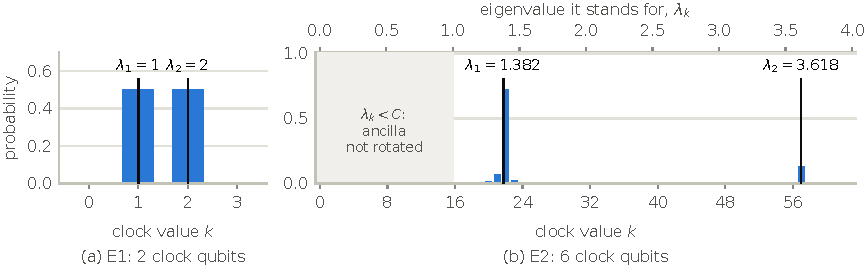
\includegraphics[width=\linewidth]{figures/fig_clock}
  \caption{Contents of the clock register after phase estimation. (a) In E1
    the two eigenvalues fall exactly on clock values. (b) In E2 the eigenvalue
    $\lambda_1$ falls between two clock values and spreads over its
    neighbours. The vertical lines mark the true eigenvalues, which the
    algorithm is never told. In the shaded region the ancilla is not
    rotated.}
  \Description{Two bar charts of probability against clock value. The left
    chart has four clock values with bars of height 0.5 at values 1 and 2.
    The right chart has 64 clock values with a tall bar at 22 flanked by
    small bars, and a single bar of height 0.13 at 57. A shaded band covers
    clock values 0 to 15.}
  \label{fig:clock}
\end{figure}

\subsection{E2: a coupled system with unknown eigenvalues}
\label{sec:e2}

For E2 the code is given only the matrix and the right-hand side. It derives
$C=1$ and $\Lambda=4$ from the Gershgorin intervals, sets $t=\ETwoT$ by
Eq.~\eqref{eq:tchoice} and uses \ETwoNClock{} clock qubits, so neighbouring
clock values are \ETwoResolution{} apart. Figure~\ref{fig:clock}b shows what
phase estimation finds. The larger
eigenvalue happens to fall almost on a clock value ($k=\ETwoClockHigh$) and
appears as a single bar. The smaller one falls at $k=\ETwoClockLow$: the
nearest clock value \ETwoPeakClock{} receives probability
\ETwoPeakProbability{} and the rest spreads over the neighbours. Reading the
histogram against the upper axis gives the eigenvalues to two digits. This is
the sense in which HHL works ``without knowing the eigenvalues'': the clock
register measures them on the fly.

The consequence of the spreading is visible in Table~\ref{tab:small}. Even
without shot noise the circuit returns $(2.570,\,2.179)$ where the classical
solution is $(2.6,\,2.2)$, an error of \ETwoRelErrExact\,\% of $\norm{x}$. Both
entries are about 1\,\% low, so the direction of the solution is nearly
perfect (fidelity \ETwoFidelity) and the error sits almost entirely in the
norm, which is recovered from a success probability of \ETwoSuccessExact{}
instead of the ideal \ETwoSuccessIdeal. The sampled values of both frameworks scatter around
the exact circuit values as the error bars predict, and the positive
$\langle X\rangle$ with vanishing $\langle Y\rangle$ confirms that both
displacements have the same sign.

\subsection{E3 and E4: larger systems}
\label{sec:e3}

\begin{table}[t]
  \caption{Results of the experiments with a two-qubit memory. Columns as in
    Table~\ref{tab:small}. The padding state of E4 is the fourth basis state
    of the memory, which does not correspond to any block.}
  \label{tab:large}
  \small
  \begin{tabular}{lcccc}
\toprule
 & Classical & Circuit, exact & Cirq, 8192 shots & Qiskit, 8192 shots \\
\midrule
\multicolumn{5}{l}{\textit{E3: chain of four blocks}} \\
$x_1$ & $0.600$ & $0.597$ & $0.576 \pm 0.011$ & $0.574 \pm 0.011$ \\
$x_2$ & $0.800$ & $0.796$ & $0.800 \pm 0.010$ & $0.792 \pm 0.010$ \\
$x_3$ & $0.800$ & $0.796$ & $0.791 \pm 0.010$ & $0.823 \pm 0.010$ \\
$x_4$ & $0.600$ & $0.597$ & $0.604 \pm 0.011$ & $0.598 \pm 0.011$ \\
$\lVert x\rVert$ & $1.414$ & $1.407$ & $1.401 \pm 0.008$ & $1.411 \pm 0.008$ \\
success probability & $0.500$ & $0.495$ & $0.491 \pm 0.006$ & $0.498 \pm 0.006$ \\
\midrule
\multicolumn{5}{l}{\textit{E4: chain of three blocks}} \\
$x_1$ & $0.381$ & $0.381$ & $0.385 \pm 0.005$ & $0.382 \pm 0.005$ \\
$x_2$ & $0.143$ & $0.143$ & $0.139 \pm 0.005$ & $0.131 \pm 0.005$ \\
$x_3$ & $0.048$ & $0.050$ & $0.059 \pm 0.006$ & $0.054 \pm 0.006$ \\
padding state & $0$ & $0.000$ & 0 counts & 0 counts \\
$\lVert x\rVert$ & $0.410$ & $0.410$ & $0.414 \pm 0.005$ & $0.407 \pm 0.005$ \\
success probability & $0.168$ & $0.168$ & $0.171 \pm 0.004$ & $0.166 \pm 0.004$ \\
\bottomrule
\end{tabular}

\end{table}

\begin{figure}[t]
  \centering
  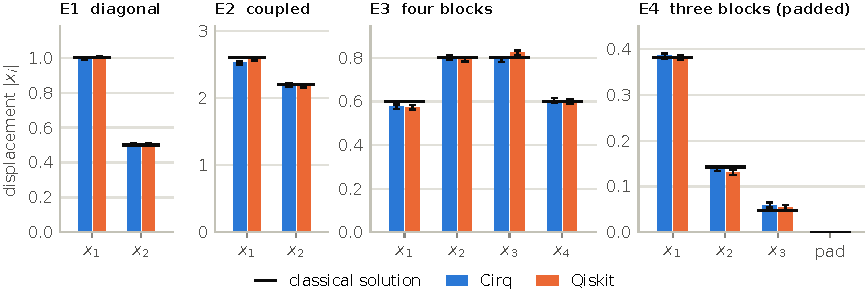
\includegraphics[width=\linewidth]{figures/fig_results}
  \caption{Displacements decoded from \Shots{} shots in Cirq and Qiskit,
    compared with the classical solution (black lines). Error bars show one
    standard error.}
  \Description{Four bar charts, one per experiment, with one pair of bars per
    unknown. In every chart the Cirq and Qiskit bars reach the black line
    that marks the classical solution to within the error bars. The fourth
    chart has an empty group for the padding state.}
  \label{fig:results}
\end{figure}

Nothing in either program is specific to $2\times 2$ matrices, so the
step to a two-qubit memory only changes the input. For the chain of four
blocks (E3) the uniform load is encoded by $R_y(\pi/2)$ on both memory qubits,
and the Gershgorin bounds are $[1,5]$. With six clock qubits the exact circuit
output is within \EThreeRelErrExact\,\% of the classical solution
$(0.6,\,0.8,\,0.8,\,0.6)$, and the sampled values reproduce the symmetric
profile of the chain (Table~\ref{tab:large}, Figure~\ref{fig:results}).

E4 exercises padding. The $3\times 3$ chain is embedded in a $4\times 4$
matrix, and the fourth basis state of the memory is never observed in either
framework, as it should be. E4 also shows the read-out problem in miniature.
The third displacement is only $0.048$, less than ten times the uncertainty
$\norm{b}/(2C\sqrt S)=\EFourErrorBar$ that Eq.~\eqref{eq:errorbar} assigns to
every entry, and with a success probability of \EFourSuccessExact{} only about
one shot in six is accepted. Its sampled values carry a relative uncertainty of
about 10\,\%, while the largest entry is known to about 1\,\%. Over all four experiments
the largest deviation between a sampled entry and the exact circuit value is
\WorstSigma{} standard errors among \NumSampledComponents{} entries, as
expected for statistical scatter. Table~\ref{tab:summary} summarises the
algorithmic accuracy and the size of the four circuits.

\begin{table}[t]
  \caption{Summary of the four circuits. Success probability, fidelity and
    relative error are exact (state vector) values; gate counts refer to the
    Qiskit circuit compiled to CNOT and single-qubit gates.}
  \label{tab:summary}
  \small
  \begin{tabular}{lcccc}
\toprule
 & E1 & E2 & E3 & E4 \\
\midrule
Qubits & 4 & 8 & 9 & 9 \\
Success probability & $0.625$ & $0.454$ & $0.495$ & $0.168$ \\
Fidelity with the classical solution & $1.0000$ & $0.9998$ & $0.9997$ & $0.9972$ \\
Relative error of $|x|$ & 0.00\,\% & 1.07\,\% & 0.51\,\% & 0.68\,\% \\
CNOT gates after compilation & 20 & 166 & 238 & 262 \\
Circuit depth after compilation & 37 & 243 & 370 & 418 \\
\bottomrule
\end{tabular}

\end{table}

\subsection{Accuracy and cost versus clock size}
\label{sec:sweep}

\begin{figure}[t]
  \centering
  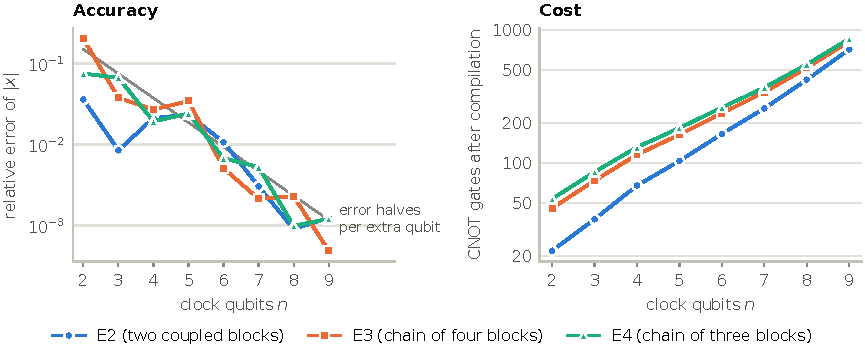
\includegraphics[width=\linewidth]{figures/fig_sweep}
  \caption{Left: relative error of the exact circuit output,
    $\norm{\,|x_{\mathrm{HHL}}|-|x|\,}/\norm{x}$, against the number of clock
    qubits. Right: CNOT gates of the compiled Qiskit circuit.}
  \Description{Two line charts against the number of clock qubits from 2 to
    9. In the left chart the relative error of three experiments falls from
    between 4 and 20 percent to about 0.1 percent, following a straight
    guide line on the logarithmic scale that halves with every qubit. In the
    right chart the number of CNOT gates rises from about 20 to 50 up to
    about 700 to 900.}
  \label{fig:sweep}
\end{figure}

How many clock qubits are enough? Figure~\ref{fig:sweep} repeats E2 to E4 for
$n=2,\dots,\SweepMaxClock$ and plots the error of the exact circuit output, so
that shot noise plays no role. The curves are not smooth, because the error
depends on where the eigenvalues happen to fall between clock values, and that
changes with $n$. The trend is clear nevertheless: a least-squares fit gives a
reduction by a factor of \ETwoErrorFactor{} (E2), \EThreeErrorFactor{} (E3) and
\EFourErrorFactor{} (E4) per additional qubit, that is, the error roughly
halves. This is the $1/\epsilon$ in the running time of HHL seen from the
other side: one more bit of accuracy needs one more clock qubit, and the
longest evolution $U^{2^{n-1}}$ doubles.

The price is on the right of Figure~\ref{fig:sweep}. Between six and nine
clock qubits the CNOT count of the compiled circuit grows by a factor of
\ETwoCxGrowth{} (E2), \EThreeCxGrowth{} (E3) and \EFourCxGrowth{} (E4) per
qubit, heading towards 2, because the look-up rotation has one angle per clock
value. For E2 the error
falls from \ETwoRelErrFour\,\% at four clock qubits (\ETwoCxFour{} CNOTs) to
\ETwoRelErrEight\,\% at eight (\ETwoCxEight{} CNOTs). A rotation that computes
$\arcsin(C/\lambda)$ with quantum arithmetic instead of a table would avoid
the exponential growth, at the cost of a far more complex circuit.

\section{Discussion}
\label{sec:discussion}

\subsection{Lessons for the next student}

\emph{Fix the conventions before writing gates.} Bit order and the sign of
the evolution have to match the Fourier transform. A mismatch does not raise
an error; with the wrong sign the clock simply holds $2^n-k$ instead of $k$
and every eigenvalue is inverted as if it were a different one.
Table~\ref{tab:conventions} is the table we wish we had started with.

\emph{Distrust default arguments.} The mistake in the textbook example is one
missing keyword. The program ran, produced plausible numbers and was printed.
Comparing with a classical solution is what exposes it.

\emph{Look at the clock register first.} A histogram like
Figure~\ref{fig:clock} can be produced after stage~2 alone. If its peaks are
not where the eigenvalue bounds say they should be, nothing after it can work,
and the histogram says whether $t$, the bit order or the sign is at fault.

\emph{Separate the two kinds of error.} The state vector shows the error of
the algorithm; sampling adds shot noise on top. Looking only at sampled
results, the 1\,\% bias of E2 and a statistical fluctuation are
indistinguishable.

\emph{Choose $C$ on purpose.} The default of the listing is safe but makes the
success probability collapse as the clock grows. Any lower bound on the
eigenvalues is better.

\emph{A fixed seed is not always enough.} Rebuilding this paper from scratch
changed one sampled number although every seed was fixed. The cause was the
compilation step in front of the Qiskit simulator: with its default settings
the transpiler re-synthesises groups of gates and chooses among equivalent
decompositions at random, and the simulator then draws a different, equally
valid sample. Compiling with \code{optimization\_level=0} removed the
variation. We only found this because we rebuilt everything twice and compared
the results file byte by byte.

\subsection{Limitations}

Our circuits contain $e^{iAt}$ as a ready-made matrix, computed classically,
and therefore demonstrate the logic of HHL, not its speed. The matrices are
positive definite; negative eigenvalues would require reading the upper half
of the clock values as negative numbers. The parameter recipe depends on a
positive Gershgorin bound, which not every matrix offers. The read-out of
Section~\ref{sec:readout} recovers magnitudes only and needs a number of shots
that grows with the number of entries one wants to know. Finally, the
simulations are noiseless. The compiled circuits contain between \EOneCx{} and
\EFourCx{} CNOT gates (Table~\ref{tab:summary}), and we have not tested how
they would fare on hardware.

\section{Conclusion}

We built the HHL algorithm in Cirq and in Qiskit and used it to solve four
small linear systems. Starting from a textbook listing forced us to understand
every line of it: repairing it for a current Cirq release uncovered an
unpassed argument that explains why the numbers printed in the book do not
match the numbers the listing itself expects. The two implementations use
opposite conventions in almost every respect and still agree to machine
precision, which is the strongest test we have. With eigenvalue bounds from
the Gershgorin theorem in place of the eigenvalues, six clock qubits are
enough to recover the solutions of all four systems to about 1\,\% before
shot noise, and every further clock qubit halves the error while the look-up
rotation makes the circuit about one and a half times as large. Natural next
steps are to replace the classically computed evolution by a genuine
Hamiltonian simulation, to add amplitude amplification, and to run the
four-qubit circuit of E1 on real hardware.

\begin{acks}
\textbf{Use of AI.} The assignment allows AI help for the Qiskit
implementation, with attribution. Claude, a large language model by
Anthropic~\cite{claude2026}, was used to write the Qiskit implementation. It
was also used to port the textbook listing to the current Cirq release, to
write the experiment, plotting and test scripts, and to prepare a first draft
of this text. The Cirq code starts from Listing~5.1 of
Pattanayak~\cite{pattanayak2021}. The author is responsible for the final
content.
\end{acks}

\bibliographystyle{ACM-Reference-Format}
\bibliography{references}

\appendix

\section{Reproducing the results}
\label{app:reproduce}

The supplementary archive contains the code, the unmodified textbook files
and this paper's \LaTeX{} source. With Python~3.11 or newer:
\begin{lstlisting}[language=bash,frame=none]
pip install cirq-core qiskit qiskit-aer matplotlib pylatexenc pytest
cd code
pytest -q                      # automated checks
python run_experiments.py      # all experiments -> ../results/results.json
python make_paper_assets.py    # figures, tables and numbers for the paper
python textbook_replay.py      # runs the original textbook files unmodified
\end{lstlisting}

\section{Source code}
\label{app:code}

The three modules below are complete. The scripts that run the experiments
and produce the figures are part of the supplementary archive.

\lstinputlisting[caption={\code{hhl\_common.py}: test systems, parameter
  choice, rotation angles and decoding.},label={lst:common}]{code/hhl_common.py}

\lstinputlisting[caption={\code{hhl\_cirq.py}: the Cirq implementation, ported
  from the textbook listing.},label={lst:cirqfull}]{code/hhl_cirq.py}

\lstinputlisting[caption={\code{hhl\_qiskit.py}: the Qiskit
  implementation.},label={lst:qiskitfull}]{code/hhl_qiskit.py}

\end{document}
